\documentclass[12pt, titlepage]{article}
\usepackage{../../project_latex/report-style}

\usepackage{fullpage}
\usepackage[round]{natbib}
\usepackage{multirow}
\usepackage{booktabs} 
\usepackage{tabularx}
\usepackage{graphicx}
\usepackage{float}
\usepackage{hyperref}
\hypersetup{
    colorlinks,
    citecolor=black,
    filecolor=black,
    linkcolor=red,
    urlcolor=blue
}
\usepackage[round]{natbib}

\newcounter{acnum}
\newcommand{\actheacnum}{AC\theacnum}
\newcommand{\acref}[1]{AC\ref{#1}}

\newcounter{ucnum}
\newcommand{\uctheucnum}{UC\theucnum}
\newcommand{\uref}[1]{UC\ref{#1}}

\newcounter{mnum}
\newcommand{\mthemnum}{M\themnum}
\newcommand{\mref}[1]{M\ref{#1}}

\title{SE 3XA3: Software Requirements Specification\\Title of Project}

\author{Team \#, Team Name
		\\ Dawson Myers mysersd1
		\\ Brandon Roberts roberb1
		\\ Yang Liu liuy136
}

\date{\today}

%\input{../../Comments}



%------------------------------------------------------------------------------
%------------------------------------------------------------------------------
% Document Info
%------------------------------------------------------------------------------
%------------------------------------------------------------------------------
\newcommand{\docTitle}{Module Guide}
\newcommand{\dueDate}{November 10, 2017}


%------------------------------------------------------------------------------
%------------------------------------------------------------------------------
% Revision Table
%------------------------------------------------------------------------------
%------------------------------------------------------------------------------
\newcommand{\revisionTable}{
	\begin{table}[hp]
		
		\begin{tabularx}{\textwidth}{p{3cm}p{2cm}X}
			\toprule {\bf Date} & {\bf Version} & {\bf Notes}\\
			\midrule
			
			10-Nov-2017 & 0.0 & Revision 0\\
			
			\bottomrule
		\end{tabularx}
		\caption{\bf Revision History}
	\end{table}
}




% Header
%-------------------------------------------------------------------------------
\usepackage{afterpage}
\usepackage{fancyhdr}
\pagestyle{fancy}
\setlength{\headheight}{15pt}
%\fancyhead[LE,RO]{\slshape \rightmark}
%\fancyhead[LO,RE]{\slshape \leftmark}
\fancyhead[LE,RO]{\slshape Assignment 1}
\fancyhead[LO,RE]{\slshape \leftmark}
\fancyfoot[C]{\thepage}
%\headrulewidth 0.4pt
%\footrulewidth 0 pt

\fancyhead{} % clear all header fields
%\fancyhead[RO,LE]{\textbf{\docTitle}}
\fancyhead[C]{\textbf{\docTitle}}
\fancyfoot{} % clear all footer fields
\fancyfoot[LE,RO]{\thepage}
\fancyfoot[LO,CE]{\dueDate}
%\fancyfoot[CO,RE]{\textbf{\teamname}}
\fancyfoot[CO,RE]{\teamname}
\renewcommand{\headrulewidth}{0.4pt}
%\renewcommand{\footrulewidth}{0.4pt}
\setlength{\headsep}{0.2in}

\begin{document}

%\maketitle
%
%\pagenumbering{roman}
%\tableofcontents
%\listoftables
%\listoffigures
%
%\begin{table}[bp]
%\caption{\bf Revision History}
%\begin{tabularx}{\textwidth}{p{3cm}p{2cm}X}
%\toprule {\bf Date} & {\bf Version} & {\bf Notes}\\
%\midrule
%Date 1 & 1.0 & Notes\\
%Date 2 & 1.1 & Notes\\
%\bottomrule
%\end{tabularx}
%\end{table}
%
%\newpage
%
%\pagenumbering{arabic}


	%------------------------------------------------------------------------------
%------------------------------------------------------------------------------
%	Title Page
%------------------------------------------------------------------------------
%------------------------------------------------------------------------------


\begin{titlepage}

%------------------------------------------------------------------------------
%------------------------------------------------------------------------------
%	Document Information
%------------------------------------------------------------------------------
%------------------------------------------------------------------------------

% Team Info
\newcommand{\teamname}{REST Assured}
\newcommand{\teamnumber}{Team 31}

% Project Info
\newcommand{\course}{SE 3XA3}

% \docTitle defined in main tex doc
\title{\course: \docTitle \\ \teamname}

% Student 1
\newcommand{\studentAname}{Dawson Myers}
\newcommand{\studentAsid}{400005616}
\newcommand{\studentAmid}{myersd1}
\newcommand{\studentAInfo}{\studentAname \studentAsid \studentAmid}

% Student 2
\newcommand{\studentBname}{Yang Liu}
\newcommand{\studentBsid}{400038517}
\newcommand{\studentBmid}{liuy136}
\newcommand{\studentBInfo}{\studentBname \studentBsid \studentBmid}

% Student 3
\newcommand{\studentCname}{Brandon Roberts}
\newcommand{\studentCsid}{400018117}
\newcommand{\studentCmid}{roberb1}
\newcommand{\studentCInfo}{\studentCname \studentCsid \studentCmid}


\author{\teamnumber
	\\ \teamname
	\\ \studentAInfo
	\\ \studentBInfo
	\\ \studentCInfo
	%\\ Dawson Myers 400005616  mysersd1
	%\\ Yang Liu 400038517 liuy136
	%\\ Brandon Roberts 400018117 roberb1
}

\date{\dueDate}


%\maketitle

\centering
\parbox[t]{0.97\linewidth}{
	\centering \fontsize{20pt}{25pt}\selectfont % The first argument for fontsize is the font size of the text and the second is the line spacing

	\Large \course \\
	\huge \teamname \\
	\large\dueDate
	
	\vspace{0.1in}
	\hrule
	\vspace{0.1in}
	
	\Huge \docTitle
	
	\vspace{0.05in}
	\hrule
	\vspace{0.4in}
	
	\large \teamnumber
	
	\vspace{0.1in}
}

% Team member info
%-------------------------------------------------------------------------------
\begin{minipage}[c]{\linewidth}
%\fontsize{14pt}{25pt}\selectfont
			\large
			\centering
			\begin{tabular}{l c c}
				\studentAname & \studentAmid & \studentAsid \\
				\studentBname & \studentBmid & \studentBsid \\
				\studentCname & \studentCmid & \studentCsid \\
			\end{tabular}
\end{minipage}

%\vfill

%% Revision table
%%-------------------------------------------------------------------------------
%\begin{table}[bp]
%	\caption{\bf Revision History}
%	\begin{tabularx}{\textwidth}{p{3cm}p{2cm}X}
%		\toprule {\bf Date} & {\bf Version} & {\bf Notes}\\
%		\midrule
%		
%		06-Oct-2017 & 0.0 & Revision 0\\
%
%		\bottomrule
%	\end{tabularx}
%\end{table}

%\revisionTable

\end{titlepage}


%------------------------------------------------------------------------------
%------------------------------------------------------------------------------
%	Report
%------------------------------------------------------------------------------
%------------------------------------------------------------------------------

\pagenumbering{roman}
\def\thesection{\arabic{section}} 
\renewcommand\thesection{\arabic{section}} 
\renewcommand\thesubsection{\thesection.\arabic{subsection}}

\tableofcontents

\listoftables

\listoffigures


\newpage

\pagenumbering{arabic}
%==============================================================================
\section{Revision History}
%==============================================================================
\revisionTable


%==============================================================================
\section{Introduction}
%==============================================================================

\subsection{Context}

The Module Guide (MG)’s purpose is to decompose the system into modules to present its modular structures. The MG’s creation is guided by principles and patterns, following the creation of the Software Requirements Specification, which specified functional and nonfunctional requirements to be implemented for the reconstruction of the Sails Live Chrome app, named the REST Assured Test Client. The MG serves in part to demonstrate how the system meets the functional and nonfunctional requirements specified in the SRS. The MG prepares the foundation for the MIS, which states the syntax of all exported routines (inputs, outputs, and exceptions), and semantics (state variables, environment variables, assumptions and special considerations, and access routine semantics) in more detail for the modules specified in the MG.  

\subsection{Audience} 

The MG is aimed to provide information for three potential groups of audience:

\begin{itemize}
\item Designers/developers: The MG provides module specifications and the traceback to requirements to ensure designers and developers can check for consistency and feasibility, and determine how the project satisfies the requirements specified. 

\item New project members: The MG provides guidance for any onboarding project member to understand the project’s big picture and to be able to quickly locate desired relevant information. 

\item Maintainers: The MG provides guidance for future maintenance for any anticipated changes. By the outline of the module hierarchy and interpretation of the uses relationships, maintainers are able to infer risk factors and better assess aspects involved in potential changes to the system. Note it is assumed that maintainers hold the responsibility to update relevant sections after making changes.
\end{itemize}

\subsection{Design Principles} 

Several design principles were used to guide the decomposition of the system into modules, these include information hiding and encapsulation, design for change, low coupling / high cohesion, and avoidance of the existence of cycles in the uses relation hierarchy. The principle of information hiding ensures that modules each holds a secret hidden from the system (for example, the file storage module hides I/O access). The principle of encapsulation ensures that the module interface remains the same (providing the same service to the system) even if the implementation details may change. Designing for change allows the design to be flexible and reusable. Low coupling / high cohesion ensures different modules are not interdependent on one another and that all components of each module are grouped together to contribute to a single well-defined goal of the module. Elimination of cycles in the uses relation ensures modules are not cyclically interdependent and thus do not cause errors or infinite loops.

\subsection{Document Structure}

The MG is organized with the following structure:

\begin{itemize}
\item [Section 3]
Anticipated and Unlikely Changes to the system’s implementation used for the traceability matrices.
\item [Section 4]
Module Hierarchy details all the modules and their hierarchy by secrets.
\item [Section 5]
Connection Between Requirements and Design details the relationship between the requirements to modules.
\item [Section 6]
Module Decomposition details the module name, secret, and service/responsibility.
for each module.
\item [Section 7]
Traceability Matrices provide details on the connection from the requirements to the modules.
\item [Section 8]
Uses Hierarchy between Modules details the uses relations interrelationships between modules.
\end{itemize}




\hypertarget{Decomposing}{Decomposing} a system into modules is a commonly accepted approach to developing.
software.  A module is a work assignment for a programmer or programming
team.  We advocate a decomposition
based on the principle of information hiding.  This principle supports design for change, because the ``secrets'' that each module
hides represent likely future changes.  Design for change is valuable in SC,
where modifications are frequent, especially during initial development as the
solution space is explored.

Our design follows the rules laid out by Parnas, as follows:
\begin{itemize}
\item System details that are likely to change independently should be the
  secrets of separate modules.
\item Each data structure is used in only one module.
\item Any other program that requires information stored in a module's data
  structures must obtain it by calling access programs belonging to that module.
\end{itemize}

After completing the first stage of the design, the Software Requirements
Specification (SRS), the Module Guide (MG) is developed. The MG
specifies the modular structure of the system and is intended to allow both
designers and maintainers to easily identify the parts of the software.  


The rest of the document is organized as follows. 
\begin {itemize}
\item [Section \ref{SecChange}] lists the anticipated and unlikely changes of the software
requirements. 
\item [Section \ref{SecMH}] summarizes the module decomposition that
was constructed according to the likely changes. 
\item [Section \ref{SecConnection}]
specifies the connections between the software requirements and the
modules. 
\item [Section \ref{SecMD}]
gives a detailed description of the
modules. 
\item [Section \ref{SecTM}]
includes two traceability matrices. One checks
the completeness of the design against the requirements provided in the SRS. The
other shows the relation between anticipated changes and the modules. Section\item [Section \ref{SecUse}] 
the use relation between modules.
\end {itemize}
%==============================================================================
\section{Anticipated and Unlikely Changes} \label{SecChange}
%==============================================================================

This section lists possible changes to the system. According to the likeliness
of the change, the possible changes are classified into two
categories. Anticipated changes are listed in Section \ref{SecAchange}, and
unlikely changes are listed in Section \ref{SecUchange}.

\subsection{Anticipated Changes} \label{SecAchange}
%------------------------------------------------------------------------------
Anticipated changes are the source of the information that is to be hidden
inside the modules. Ideally, changing one of the anticipated changes will only
require changing the one module that hides the associated decision. The approach
adapted here is called design for
change.

\begin{description}
\item[\refstepcounter{acnum} \actheacnum \label{acHardware}:] The format of the output data.
\item[\refstepcounter{acnum} \actheacnum \label{acInput}:] The format of the input parameters.
\item[\refstepcounter{acnum} \actheacnum \label{acSettings}:] The default settings.
\item[\refstepcounter{acnum} \actheacnum \label{acData}:] The implementation of the data structure that stores JSON profile.
\item[\refstepcounter{acnum} \actheacnum \label{acgui}:] The graphical user interface elements used to retrieve user input and their format.
\end{description}

\subsection{Unlikely Changes} \label{SecUchange}
%------------------------------------------------------------------------------
The module design should be as general as possible. However, a general system is
more complex. Sometimes this complexity is not necessary. Fixing some design
decisions at the system architecture stage can simplify the software design. If
these decision should later need to be changed, then many parts of the design
will potentially need to be modified. Hence, it is not intended that these
decisions will be changed.

\begin{description}
\item[\refstepcounter{ucnum} \uctheucnum \label{ucIO}:] Input/Output devices (Input: File and/or Keyboard, Output: File, Memory, and/or Screen).
\item[\refstepcounter{ucnum} \uctheucnum \label{ucInput}:] Storage method of output data.
\item[\refstepcounter{ucnum} \uctheucnum \label{ucInput}:] There will always be a source of input data external to the software.
\end{description}

%==============================================================================
\section{Module Hierarchy} \label{SecMH}
%==============================================================================
This section provides an overview of the module design. Modules are summarized
in a hierarchy decomposed by secrets in Table \ref{TblMH}. The modules listed
below, which are leaves in the hierarchy tree, are the modules that will
actually be implemented.

\begin{description}
\item [\refstepcounter{mnum} \mthemnum \label{mHH}:] Hardware-Hiding Module
\item ...
\end{description}


\begin{table}[h!]
\centering
\begin{tabular}{p{0.3\textwidth} p{0.6\textwidth}}
\toprule
\textbf{Level 1} & \textbf{Level 2}\\
\midrule

{Hardware-Hiding Module} & ~ \\
\midrule

\multirow{7}{0.3\textwidth}{Behaviour-Hiding Module}
& Input Module\\
& Request Testing Module\\
& User Profile Module\\
& Data Processing Module\\
& Network Module\\
& Output Module\\
\midrule

\multirow{3}{0.3\textwidth}{Software Decision Module}\\
& Request Test Structure Module\\
& Test Flow Structure Module\\
\midrule
{Module Name} & {Module Number}\\
\midrule
Input Module & M1\\
Request Testing Module & M2\\
User Profile Module & M3\\?
Data Processing & M4\\
Network Module & M5\\
Test Flow Module & M6\\
Request Test Structure Module & M7\\
Output Module & M8\\
\bottomrule

\end{tabular}
\caption{Module Hierarchy}
\label{TblMH}
\end{table}
\newpage

%==============================================================================
\section{Connection Between Requirements and Design} \label{SecConnection}
%==============================================================================
The design of the system aims to satisfy the requirements specified in the SRS. The decomposition of the system into component modules analyzes the connection between requirements and modules, which is detailed in the Traceability Matrices section below. To satisfy requirements, several design decisions were made with design principles in mind to guide the decomposition of the system into modules. The I/O class handles input and output of data storage and is used by other modules for this purpose to meet functional requirements, thus demonstrating the design principle of information hiding and encapsulation. The application class RestSuite connects all components in the system to ensure the program can be executed. Nonfunctional requirements related to appearance and usability are satisfied in the RestSuite.display module, since it handles user interaction and interface functions and capabilities. The programming language selected (JavaScript) enables cross-platform support of the application by using the Chrome JavaScript runtime, making it platform agnostic. Another design decision was to implement a drop down menu for the selection of the type of REST requests, which eliminates invalid input and contribute to an intuitive usability design. In addition, buttons are utilized to further simplify request submission for the user. These design decisions holistically contribute to ensure the meeting of the cultural requirements.
\ref{TblRT}.


%==============================================================================
\section{Module Decomposition} \label{SecMD}
%==============================================================================

Modules are decomposed according to the principle of ``information hiding''
proposed by Parnas. The \emph{Secrets} field in a module
decomposition is a brief statement of the design decision hidden by the
module. The \emph{Services} field specifies \emph{what} the module will do
without documenting \emph{how} to do it. For each module, a suggestion for the
implementing software is given under the \emph{Implemented By} title. If the
entry is \emph{OS}, this means that the module is provided by the operating
system or by standard programming language libraries.  Also indicate if the
module will be implemented specifically for the software.

Only the leaf modules in the
hierarchy have to be implemented. If a dash (\emph{--}) is shown, this means
that the module is not a leaf and will not have to be implemented. Whether or
not this module is implemented depends on the programming language
selected.


\subsection{Hardware Hiding Modules }
%------------------------------------------------------------------------------
\begin{description}
\item[Secrets:]The data structure and algorithm used to implement the virtual
  hardware.
\item[Services:]Serves as a virtual hardware used by the rest of the
  system. This module provides the interface between the hardware and the
  software. So, the system can use it to display outputs or to accept inputs.
\item[Implemented By:] OS
\end{description}


\subsection{Behaviour-Hiding Module}
%------------------------------------------------------------------------------
\begin{description}
\item[Secrets:]The contents of the required behaviours.
\item[Services:]Includes programs that provide externally visible behaviour of
  the system as specified in the software requirements specification (SRS)
  documents. This module serves as a communication layer between the
  hardware-hiding module and the software decision module. The programs in this
  module will need to change if there are changes in the SRS.
\item[Implemented By:] --
\end{description}


\subsubsection{Input Format Module}
%-----------------------------------------------------------
\begin{description}
\item[Secrets:]The format and structure of the input data.
\item[Services:]Converts the input data into the data structure used by the
  input parameters module.
\item[Implemented By:] RestAssured
\end{description}


\subsubsection{Input Module}
%------------------------------------------------------------------------------
\begin{description}
\item[Secrets:] Input
\item[Services:] Allows the user to specify the test conditions at which the user wishes to run tests with, the order the user wishes to run tests, and what type of tests will be performed.
\item[Implemented By:] javascript
\end{description}

\subsubsection{Request Testing Module}
%------------------------------------------------------------------------------
\begin{description}
\item[Secrets:] Test of request.
\item[Services:] Tests the success of request based on user-defined parameters.
\item[Implemented By:] javascript
\end{description}

\subsubsection{User Profile Module}
%------------------------------------------------------------------------------
\begin{description}
\item[Secrets:] User Profile Information.
\item[Services:] Keeps track of user specific settings.
\item[Implemented By:] javascript
\end{description}

\subsubsection{Data Processing Module}
%------------------------------------------------------------------------------
\begin{description}
\item[Secrets:] Data Processing
\item[Services:] Processes user input and request 	 and stores it for user and application analysis.
\item[Implemented By:] javascript
\end{description}

\subsubsection{Network Module}
%------------------------------------------------------------------------------
\begin{description}
\item[Secrets:] Network connection
\item[Services:] Performs network operations such as retrieval of remote information and interaction between computers.
\item[Implemented By:] javascript
\end{description}

\subsubsection{Output Module}
%------------------------------------------------------------------------------
\begin{description}
\item[Secrets:] Visual Text
\item[Services:]Creates multiple instances of RestStubs and outputs the response data to the screen.
\item[Implemented By:] javascript
\end{description}

\subsubsection{Request Test Structure Module}
%------------------------------------------------------------------------------
\begin{description}
\item[Secrets:] Request Test Structure
\item[Services:] Structures tests uniformly for the application to analyse.
\item[Implemented By:] javascript
\end{description}

\subsubsection{Test Flow Module}
%------------------------------------------------------------------------------
\begin{description}
\item[Secrets:] Test Flow
\item[Services:] Offers a intuitive way for the user to order tests.
\item[Implemented By:] javascript
\end{description}

\subsubsection{Etc.}
%-----------------------------------------------------------

\subsection{Software Decision Module}
%-----------------------------------------------------------

\begin{description}
\item[Secrets:] The design decision based on mathematical theorems, physical
  facts, or programming considerations. The secrets of this module are
  \emph{not} described in the SRS.
\item[Services:] Includes data structure and algorithms used in the system that
  do not provide direct interaction with the user. 
  % Changes in these modules are more likely to be motivated by a desire to
  % improve performance than by externally imposed changes.
\item[Implemented By:] --
\end{description}

\subsubsection{Etc.}


%==============================================================================
\section{Traceability Matrix} \label{SecTM}
%==============================================================================

This section shows two traceability matrices: between the modules and the
requirements and between the modules and the anticipated changes.

% the table should use mref, the requirements should be named, use something
% like fref
\begin{table}[H]
\centering
\begin{tabular}{p{0.2\textwidth} p{0.6\textwidth}}
\toprule
\textbf{Req.} & \textbf{Modules}\\
\midrule
FR1 & M1, M5, M8\\
FR2 & M1, M2, M4, M5, M8\\
FR3 & M1, M3, M4, M6, M7, M8\\

NFR1 & M1, M3, M4, M6, M7, M8\\
NFR2 & M1, M8\\
NFR3 & M1, M3, M6, M8\\
NFR4 & M1, M3, M6, M8\\
NFR5 & M1, M8\\
NFR6 & M1, M4, M5, M8\\
NFR7 & M1, M4\\
NFR8 & M1, M4\\
NFR9 & M1, M3, M6, M8\\
NFR10 &  M1, M3, M6, M8\\

\bottomrule
\end{tabular}
\caption{Trace Between Requirements and Modules}
\label{TblRT}
\end{table}

\begin{table}[H]
\centering
\begin{tabular}{p{0.2\textwidth} p{0.6\textwidth}}
\toprule
\textbf{AC} & \textbf{Modules}\\
\midrule
AC1 & M8\\
AC2 & M1\\
AC3 & M1, M3, M4, M6, M8\\
AC4 & M1, M3, M4, M8\\
AC5 & M1, M3, M4, M6, M8\\

\bottomrule
\end{tabular}
\caption{Trace Between Anticipated Changes and Modules}
\label{TblACT}
\end{table}


%==============================================================================
\section{Use Hierarchy Between Modules} \label{SecUse}
%==============================================================================

In this section, the uses hierarchy between modules is
provided. Parnas said if two programs A and B that A {\em uses} B if
correct execution of B may be necessary for A to complete the task described in
its specification. That is, A {\em uses} B if there exist situations in which
the correct functioning of A depends upon the availability of a correct
implementation of B.  Figure \ref{FigUH} illustrates the use relation between
the modules. It can be seen that the graph is a directed acyclic graph
(DAG). Each level of the hierarchy offers a testable and usable subset of the
system, and modules in the higher level of the hierarchy are essentially simpler
because they use modules from the lower levels.

\begin{figure}[H]
\centering
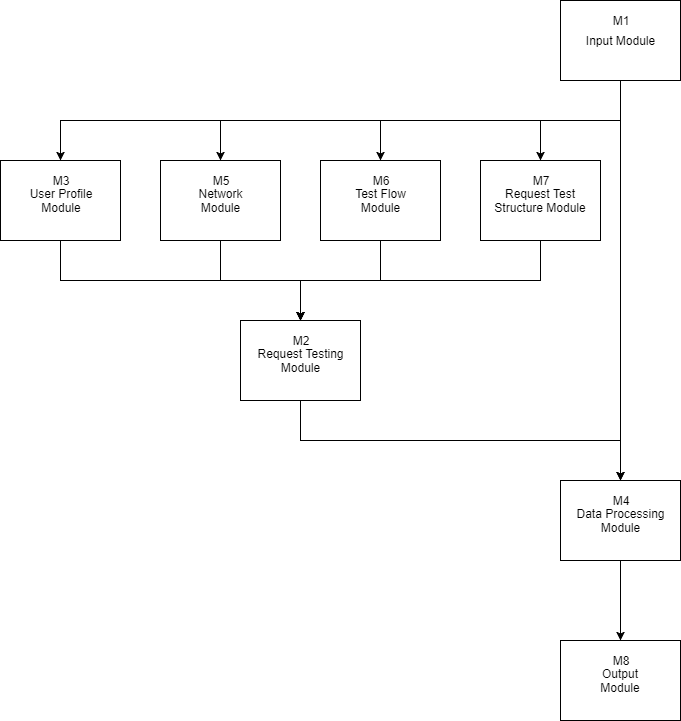
\includegraphics[width=0.7\textwidth]{UsesHierarchy.png}
\caption{Use hierarchy among modules}
\label{FigUH}
\end{figure}
\section{Gantt}
\centering
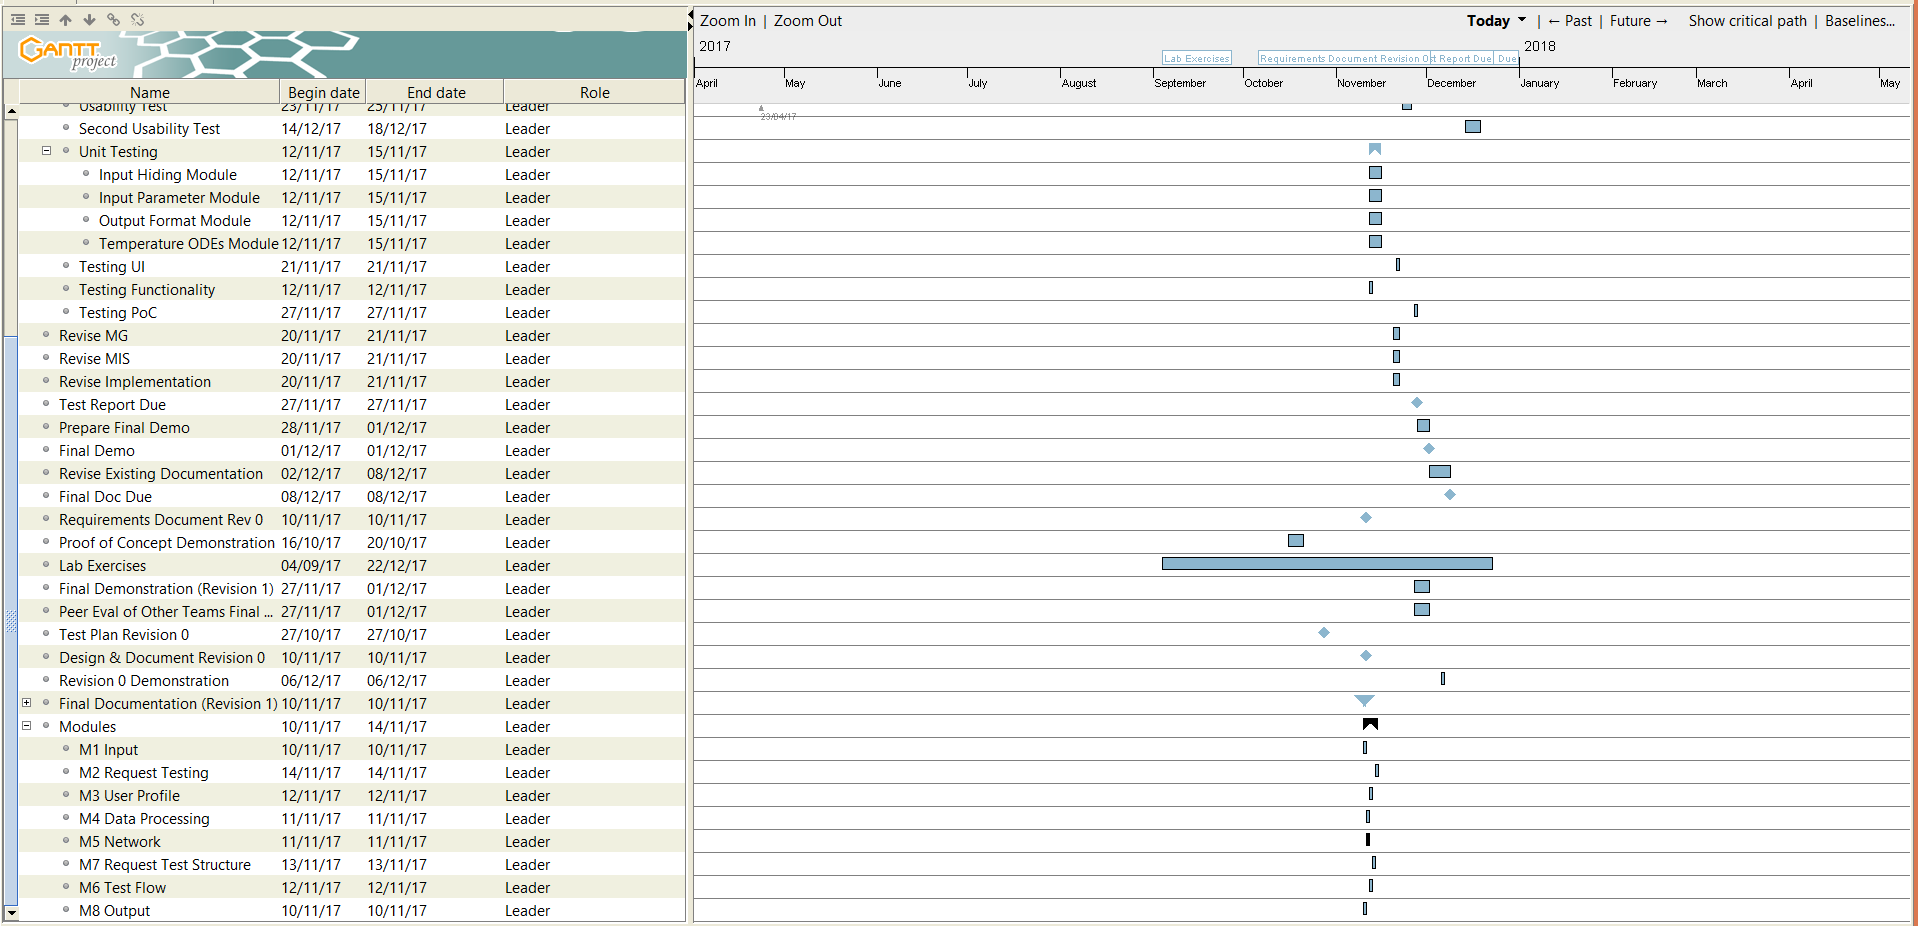
\includegraphics[width=0.7\textwidth]{gantt.png}
\newline
	See Gantt Chart at the following url: \href{https://gitlab.cas.mcmaster.ca/myersd1/3xa3-team31/blob/master/ProjectSchedule/Team%2031%20Gantt%20Project.pdf}{Team 31 Gant Project}
%\section*{References}

\bibliographystyle {plainnat}
\bibliography {MG}

\end{document}